\section{Introduction}
% Outline:
% - What is a scripting language? How do they compare to other languages?
%   - usually interpreted, or compiled on-the-fly to intermediate byte-code
%   - environments that can be automated through scripts: shells and Web browsers (perhaps the two best 
%     known examples), other general purpose examples exist such as Python; extension language: Lua
%   - "Lua is a language designed and widely used as an extension language. Python is a general-purpose 
%     language that is also commonly used as an extension language, while ECMAScript is still primarily a 
%     scripting language for web browsers, but is also used as a general-purpose language."
% - Why are they useful?
%   - "glue", cross-platform (web), rapid application development, extending application behaviour
% - Characteristics
%   - very high-level languages, high level of abstraction, dynamic
%   - dynamic: dynamically typed; interpreted; can execute code loaded over the network in the current
%     environment using an exec() method or something similar
%   - flexible type system; automatic memory managment

\lettrine[nindent=0em,lines=3]{S}{cripting} languages is an increasingly popular and important
category of programming languages. Programs written in scripting languages are often written for
a special run-time environment that can be automated through scripts--shells and Web browsers
are perhaps the two best known examples--or for a specialized domain, such as text processing.
JavaScript and Lua are examples of the former. JavaScript is used to extend the functionality
of Web pages displayed in a Web browser, while Lua is an extension language that is used in many 
commercial and free applications and is widely used in scripting video game engines. Lua is
often chosen for this task because it is designed to be very fast and easy to embed.
However, general-purpose scripting languages also exist and perhaps the most well-known one is Python.
Python is a widely-used, general-purpose high-level programming language that emphasizes code
readability and its syntax allows programmers to express concepts in fewer lines of code than would be 
possible in a language like C, enabling them to develop applications quicker. 
Scripting languages typically have a low barrier to entry and are easier for programers to 
get started with and provide a number of features that make them an important tool for increasing 
programmer productivity and distinguish them from programming languages such as C, C++ and Java. 
For example, scripting languages are generally very high-level languages that provide a high level of 
abstraction. They are usually dynamically typed and provide automatic memory management. Many
scripting languages can load and execute code dynamically in the context of the running program
by passing string consisting of program statements to an \texttt{exec()} function or something
similar.

% - basis for comparison is Letter Lizard:
%   - letter rearrangement game (show GUI mockup?)
%   - player is presented with a set of letters and the goal of the game is for the to form as
%     many words as possible from the set of letters before the timer runs out
%   - implemented in the three languages
%   - interface differs, but internal structure of the game is similar
%   - use game development framework for Python, EaselJS for JavaScript and text based UI for Lua
%   - can almost copy and paste much of our design document / proposal here

In this report, we study and compare three different scripting languages, Python,
JavaScript, and Lua, and compare the similarities and differences of the features that
they offer. Our comparison is based on the implementation of a simple letter rearrangement game
called Letter Lizard. In the game, the player is presented with a set of letters and 
their goal is to form as many dictionary words as possible from the set of letters
before the timer runs out. In order to make the game
more engaging and enjoyable, we implemented a number of features that enable the user to customize
their gameplay experience by providing options to set the number of rounds, the time per round, 
and the level of difficulty for each
game. Although wanted to create a game that is fun and enjoyable, our primary objective is to
compare and contrast the features of each programming language. Where possible, adhered to the same
design for each implementation while also using the idiomatic features of each language as much as 
possible. The game proceeds as follows:

\begin{itemize}
    \item On beginning the game, a welcome screen or a ``Splash Screen'' is displayed
    to the user. The user must hit the spacebar to proceed to the Main Menu screen.
    \item The Main Menu screen allows the user to configure game options, such as the
    number of rounds, time per round and level of difficulty. After setting the options, the
    user clicks \textbf{Start} to begin a new game and is taken to the main Game screen.
    \item The Game screen displays the set of letters to the user and allows them to type
    words that can be formed from the letters. It also shows the round number, the amount of
    time remaining, the user's score and placeholders for all of the dictionary words that
    can be formed from the set of letters. After typing a word, the user hits
    enter and the game engine checks to see that the word is a valid dictionary word, and, if so,
    reveals the word in the list of placeholders. The Game screen also has options to shuffle
    the set of letters and return to the main menu.
\end{itemize}

\begin{figure}
    \centering
    \begin{subfigure}{0.49\textwidth}
        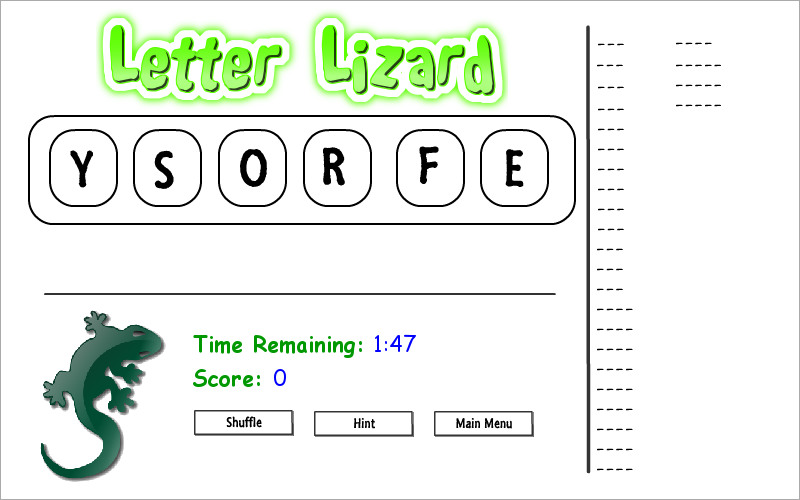
\includegraphics[width=\textwidth]{Game_Screen.jpg}
        \caption{Main game screen mockup}
        \label{mainscreenmockup}
    \end{subfigure}
    \begin{subfigure}{0.49\textwidth}
        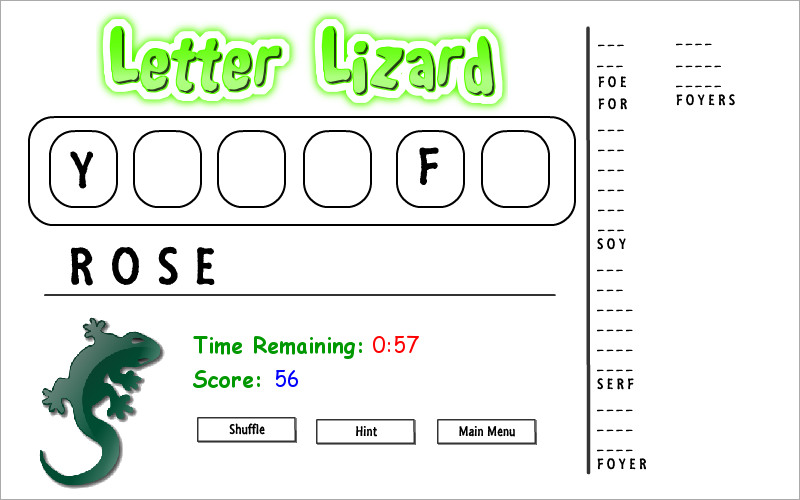
\includegraphics[width=\textwidth]{Gameplay.jpg}
        \caption{Gameplay mockup}
        \label{gameplaymockup}
    \end{subfigure}
    \caption{Two mockups from our design document demonstrating the proposed Letter Lizard game
    showing (a) the main game screen and (b) the gameplay.}
    \label{mockups}
\end{figure}

The Python and JavaScript implementations of Letter Lizard provide graphical user interfaces
that are modelled after the mockups presented in our design document. The mockups showing the
main game screen and gameplay are shown in Figure~\ref{mockups}. The Lua implementation provides
a text-based user interface\footnotemark,
but the user interaction parallels that of the other two versions.
Furthermore, the internal data structures and algorithms representing the game state and game play
are similar to the other two implementations.

\footnotetext{A ``screen'' in the text-based user interface is represented by several
lines of descriptive text printed to the console. The interface for the Lua implementation
of the game is discussed further in Section~\ref{luaimpl}.}

\paragraph{Python}
%   - modern, doesn't include "unnecessary/redundant features" (such as += or ++), or
%     features that novice programmers are likely to abuse (such as goto)
%   - talk about history, popularity, insiprational languages, main features (eg
%     more traditional object oriented class-based design)
%   - talk about major projects using Python
%   - chosen for its popularity
%   - look at Wikipedia and language website for more information


\paragraph{JavaScript}
%   - "language of the Web"
%   - history, standartization process, insiprational languages, main features (eg
%     prototype-based inheritance), variable scoping (anti-feature), "everything
%     is an object"
%   - closures
%   - chosen for its ubiquitiy
%   - look at Wikipedia and language website for more information


\paragraph{Lua}
%   - shares many similaritise with javascript
%   - minimal but powerful
%   - local variable declared only where needed, "everything is a table"
%   - designed primarily as an extensible extension language
%   - chosen becasuse it is a fast, simple, versitile languages with many advanced 
%     features (eg. operator overloading)
%   - look at Wikipedia and language website for more information
